\documentclass[pdftex]{beamer}
%\usetheme{Frankfurt}

% declare the path(s) where your graphic files are
% ../.. is the GeocronDocuments directory
\graphicspath{{../../images/external/distributed_systems/}{../../images/diagrams/}}
\DeclareGraphicsExtensions{.pdf,.png}

\begin{document}

% Show the ToC at the start of each section, with the current section highlighted
\AtBeginSection[]
{
   \begin{frame}
        \frametitle{Roadmap}
        \tableofcontents[currentsection]
   \end{frame}
}

\title[FT Comm. MW]{Fault-Tolerant Middleware: Communication}
\subtitle{Reliable communication middelware for distributed systems}
\author[K. Benson]{Kyle E. Benson}
\institute[UCI]{
  Department of Computer Science\\
  University of California, Irvine\\
  Irvine, California 92697\\[1ex]
  \texttt{kebenson@uci.edu}
}


\begin{frame}[plain]
	\titlepage
\end{frame}

% Breaking intro into its own part suppresses navigation bar info
\part{intro}

\begin{frame}{Introduction}

\begin{itemize}
	\item Fault-tolerant communication goals
	\begin{itemize}
		\item \textbf{Correctness} of messages, non-corruption guarantee
		\item \textbf{Ordering} of messages
		\begin{itemize}
			\item FIFO: If $M_a$ sent before $M_b$, $M_a$ received before $M_b$
			\item Causal: If $M_a$ causes $M_b$ to be sent, $M_a$ received before $M_b$ at all processes
			\item Total: If $M_a$ delivered before $M_b$ at process $P_j$, $M_a$ delivered before $M_b$ at all other $P_i$ too
		\end{itemize}
		\item \textbf{Delivery} guarantees, bounds on latency
	\end{itemize}
\end{itemize}
\end{frame}

% TODO: pic of msg ordering

% % % % % % % % % % % % % % % % % % % % % % % % % % % % % % % % % % % % % % % % % %
\begin{frame}{Foundations of Reliability}

\begin{itemize}
	\item How to make unicast reliable?
	\begin{itemize}
	
		\item Prevent \alert{omission failures}
		\begin{itemize}
			 \item Guarantee message delivery
			 \item Assume correct processes will deliver messages
			 \item Redeliver on \emph{timeout}
			 \item No bound on time before reply
		\end{itemize}
		
		\item Guarantee ordering; ignore repeated messages
		\begin{itemize}
			 \item Sequence numbers
			 \item Timestamps
			 \item Logical clocks
		\end{itemize}

		\item Message integrity
		\begin{itemize}
			 \item Hashing
			 \item Certificates
			 \item Keys
		\end{itemize}
	\end{itemize}
\end{itemize}
\end{frame}


% % % % % % % % % % % % % % % % % % % % % % % % % % % % % % % % % % % % % % % % % %
\begin{frame}{Reliable Group Communication}
\begin{columns}
\begin{column}{.5\textwidth}

\begin{itemize}
	\item Why not just use TCP?
	\begin{itemize}
		\item Consider 100 machines each running 10 processes
		\item 1000+ TCP connections at each machine
		\item 1 million+ total!
		\alert{\item Not scalable!}
		\item Relies on timeouts
		\item Ordering harder
		\item Similar problems with other client-server connection-oriented protocols
	\end{itemize}
	
	\item How to exploit redundancy in communication paths?
	\item Answer: multicast trees
	
\end{itemize}
\end{column}
	
\begin{column}{.5\textwidth}
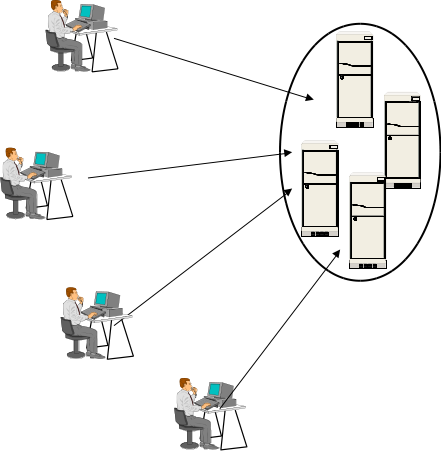
\includegraphics[width=\textwidth]{server_replica}
\end{column}

\end{columns}
\end{frame}
	
% % % % % % % % % % % % % % % % % % % % % % % % % % % % % % % % % % % % % % % % % %
\begin{frame}{Reliable Distributed Multicast}
\begin{itemize}
	\item \textbf{Observation:} distributed systems naturally address groups of processes
	\begin{itemize}
		\item Coordinating events
		\item Replica communication
		\item Anycast
		\item Reduction
		\item Parallel computation
	\end{itemize}
	
	\item Distributed process groups $\rightarrow$ multicast groups
	\begin{itemize}
		\item IP multicast not always supported
		\item Make application layer multicast
		\item Let the \emph{middleware} handle delivering message to proper groups
		\item Decouples machine address from distributed function target
	\end{itemize}
\end{itemize}
\end{frame}

% % % % % % % % % % % % % % % % % % % % % % % % % % % % % % % % % % % % % % % % % %


% % % % % % % % % % % % % % % % % % % % % % % % % % % % % % % % % % % % % % % % % %
%
%\part{rest}
%
%\begin{frame}{Roadmap}
%	\tableofcontents
%\end{frame}
%
%\section{Location Service}
%
%\begin{frame}{Location Service}
%\begin{columns}
%\begin{column}{.5\textwidth}
%
%	\begin{itemize}
%		\item Nodes have GPS
%		\item But how to look up destination's location?
%		\item Maintain global information \uncover<2->{\alert{easily outdated/inefficient}}
%		\item<3-> Distribute load
%		\begin{itemize}
%			\item In , node updates \emph{location servers} (LS) throughout network
%			\item Divide network into hierarchical grid
%			\item LS's in 3 external grids at each level
%			\item Lookup distance $<$ square LS co-resides in
%		\end{itemize}
%		
%	\end{itemize}
%
%\end{column}
%
%\begin{column}{.5\textwidth}
%\uncover<3->{
%\begin{figure}
%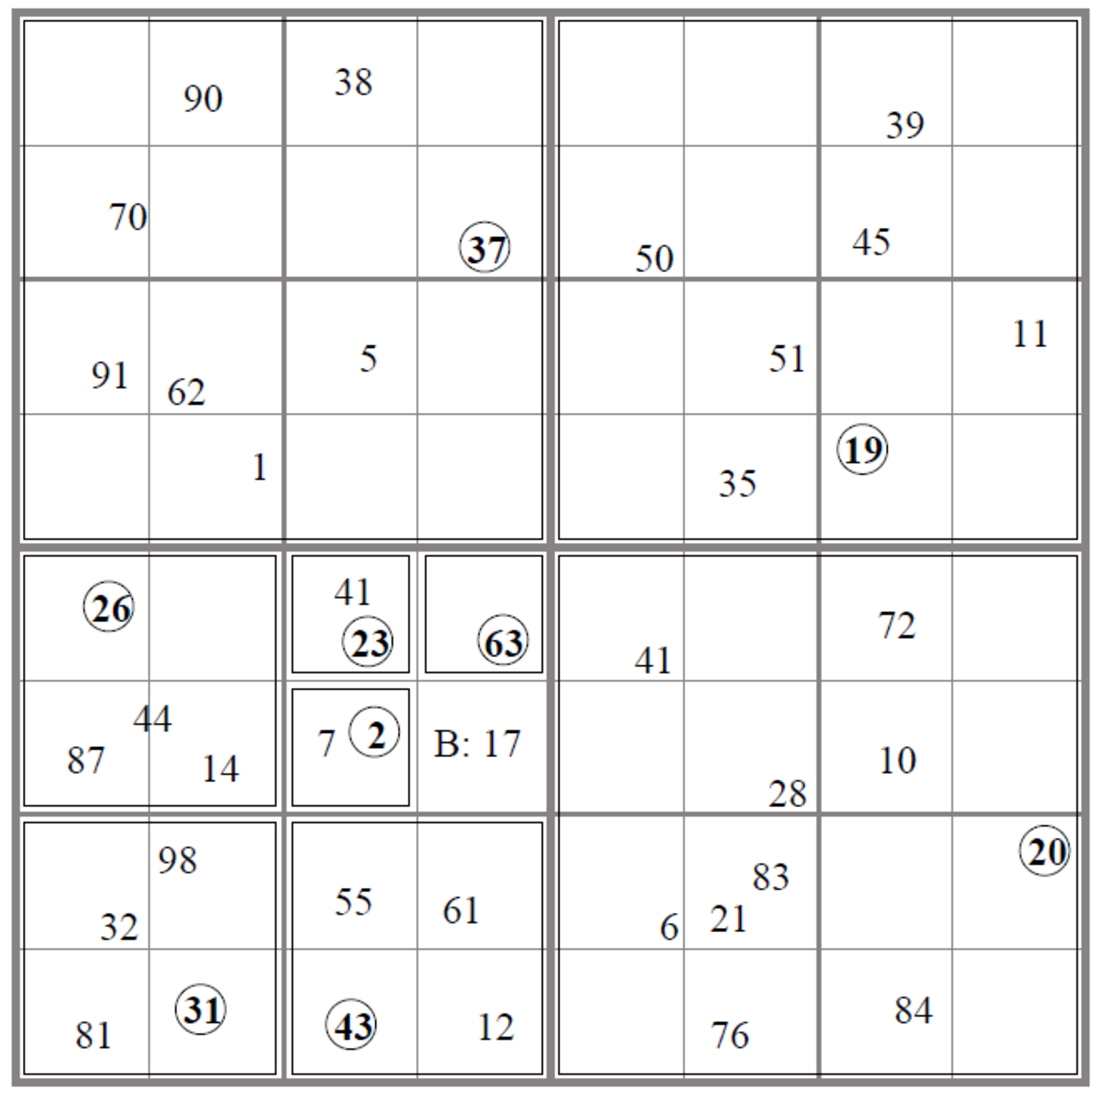
\includegraphics[width=\textwidth]{location_service}
%\caption{Hierarchical grid with 4 order-i squares in order-i+1 square.}
%\end{figure}}
%\end{column}
%\end{columns}
%\end{frame}
%

\end{document}
